\subsection*{Cornelia}
A continuación se muestra el mapa de Cornelia, pero también hay granjas y edificios más pequeños fuera de las murallas de la ciudad que no se muestran. Todos los edificios están marcados con un número y puedes encontrar más detalles sobre ellos en los párrafos numerados. El grupo llega a Cornelia desde la puerta sur, donde dos guardias los detienen ya que no reconocen a los aventureros. Aconsejan al grupo alejarse del castillo y salir de la ciudad luego de terminar sus asuntos. La mayoría de los habitantes del pueblo está demasiado asustada como para dejar sus hogares desde que la princesa ha desaparecido.
\begin{center} 
	\tcbox[left=0pt,top=0pt,right=0pt,bottom=0pt, boxsep=0pt, colframe=accent, sharp corners]{
	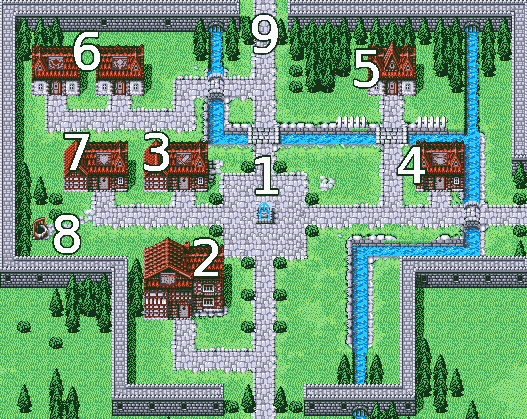
\includegraphics[width=0.98\columnwidth]{./art/maps/cornelia.png} 
	}
\end{center}
\subsubsection*{1 Fuente}
"¡Hola! ¡Soy una bailarina! ¿Qué dices? ¿Te gustaría un baile? Jijiji" -- Arylon \\ \\
El grupo observa una hermosa fuente que se destaca en medio de un pueblo por demás ordinario. En las cercanías se encuentra una joven alegre de cabello azul y vestido rojo practicando unos pasos de baile. Su nombre es Arylon. Cuando se le pregunta sobre la princesa o el castillo, revela los rumores que ha escuchado: han tomado de rehén a la princesa Sarah y piden un cuantioso rescate. En consecuencia, el castillo está inmerso en el caos y se le ha prohibido la entrada al público en general. También revela que ha habido múltiples intentos infructuosos de rescatar a Sarah. Observa las armas del grupo y les pregunta si estarían interesados en ayudar.

\subsubsection*{2. Posada}
"¡Pasen, por favor! Cobramos 50 Gil por noche. ¿Desean quedarse?" -- Elia \\\\
El grupo entra en una pequeña habitación con una alfombra roja en el suelo y un mostrador al final. Detrás del mostrador se encuentra una joven con pelo azul oscuro y un vestido largo verde. Su nombre es Elia. A la izquierda hay una amplia habitación donde los huéspedes duermen, con varias camas y pequeñas decoraciones en las paredes. A la derecha hay otra habitación, con sillas de madera y mesas donde los huéspedes pueden sentarse a comer y beber. Normalmente está sentado allí un viejo borracho llamado Argus y, a veces, unos pocos guardias. El grupo puede dormir en la posada por 50 Gil por noche por persona. También pueden pedir información a Elia, ya que escucha muchos comentarios de los visitantes. Ella le informa al grupo sobre varias personas del pueblo que pueden necesitar ayuda, como el herrero y los magos. El grupo también puede hablar con Argus, que balbuceará historias sobre un gran soldado llamado Garland que él conocía de cuándo era un guardia.

\subsubsection*{3. Herrero}
El grupo entra en una gran tienda con una forja, donde se exhiben muchas armas y armaduras. Detrás del mostrador hay un hombre viejo de pelo castaño y barba larga. Su nombre es Todo. Les dice al grupo que la tienda está cerrada: no puede trabajar debido a que no recibe la mercadería necesaria que fue enviada al puerto. Para ayudarlo, el grupo tiene que hablar con Dyce en el puerto de Cornelia, que está controlando a los envíos. El envío de Todo consiste en una caja de madera grande en un pequeño carro, que disminuye un poco el paso del grupo. En el camino de regreso, un extraño monstruo llamado PuPu intenta robar los envíos. PuPu está sentado en los árboles y utiliza su habilidad "Abducir" para hacer desaparecer lentamente la caja. Si los jugadores lo buscan en los árboles mientras él hace esto, es fácil de detectar, ya que la parte superior de su cabeza resplandece. Después de eso, es difícil de detectar: un jugador tiene que tener éxito en una tirada que puede variar entre una DC 6 y 8. Puede que el grupo no encuentre PuPu, pero estará cerca si regresan al mismo lugar en otro momento. Si se detecta, PuPu no lucha, sino que pide Pociones (consulte "¡Pociones, por favor!") y devuelve los artículos robados si el grupo las concede. También puedes recompensar al grupo por resolver la disputa pacíficamente: PuPu puede, por ejemplo, devolver artículos adicionales o Gil. El grupo también puede atacarlo, en cuyo caso el envío vuelve a aparecer después de derrotar a PuPu. Al entregar el envío, Todo recompensa al grupo con 500 Gil. El herrero puede empezar a trabajar de nuevo, pero estará ocupado completando pedidos pendientes durante algún tiempo. Cuando el grupo regrese en unos días, Todo puede mejorar sus armas o armaduras y puede vender cualquier arma o armadura de nivel 1 a elección.
\vfill
\friendly{PuPu}{???}{
\includegraphics[width=0.13\textwidth]{./art/monsters/pupu.png}}
{
	HP: & \hfill 10 & MP: & \hfill 10\\
	STR: & \hfill 0 & DEF: & \hfill 0 \\
	MAG: & \hfill 0 & RES: & \hfill 0 \\
	AGI: & \hfill 2 & Size: & \hfill S\\
}
{
	\textbf{Drops}: All abducted objects 
	
	\mtech{Abduct}{0}{1r}{Single}{5u}{
		An object that you can see within range disappears to an unknown location.  
	}{}	
	\mpassive{Potion Please!}{
		Ask your enemies to give you a \hyperlink{item}{Potion}, if they comply make a DC 8 check.
		If you succeed you disappear to an unknown location (\hyperlink{status}{KO}), otherwise you keep asking for more \hyperlink{item}{Potions}.
	}
}

\subsubsection*{4. Tienda}
Esta tienda de artículos generales está compuesta por un gran mostrador en el centro y varios objetos y productos a su alrededor. Detrás del mostrador hay un hombre joven de pelo oscuro con una bandana verde. Su nombre es Guston. No está particularmente preocupado por la princesa, pero está molesto porque los problemas en Cornelia han afectado a sus ventas. En consecuencia, es muy agradable con posibles clientes y vende los elementos que se indican a continuación. Además, puede tener cualquier otro objeto que quieras en su inventario.
%
\vspace{0.1cm}
%
\consumables{Objetos}{item2.png}{
 \hline Poción & 100 Gil & Recupera 2d de PV. \\ 
 \hline Ala de \newline Fénix & 250 Gil & Recupera el estado \hyperlink{status}{KO} y recupera 1 PV.\\ 
 \hline Carpa & 500 Gil & Permite al grupo descansar en las afueras. \\
 \hline Linterna & 100 Gil & Una linterna normal. \\ 
} 

\subsubsection*{5. Capilla}
"No pierdan el valor, valientes guerreros".
\indent -- Gregory\\\\
La capilla es pequeña y acogedora con pocos bancos de madera, pero también está completamente vacía, salvo por una persona, el padre Gregory. Gregory es un viejo de barba larga y blanca que lleva una túnica roja con capucha. Habla muy despacio y lento. Se lamenta que nadie ha visitado la capilla desde la desaparición de Sarah. Aparentemente, la mayoría de los habitantes del pueblo creen que el incidente es un castigo divino, por lo que no se acercan a la capilla. El padre le pide al grupo que restablezca la fe en el pueblo de Cornelia. El grupo puede convencer a las personas, por ejemplo, dando detalles sobre la desaparición de Sarah (fue secuestrada) que muchos no saben, ya que desde el castillo no dieron ningún tipo de información. Si el grupo consigue convencer al menos a 3 personas de Cornelia que asistan a la capilla, Gregory estará satisfecho y los recompensará con 500 Gil. Además, ofrece sus servicios de manera gratuita al grupo: puede curar el estado \hyperlink{status}{KO} realizando un ritual de 1 hora.

\subsubsection*{6. Los magos}
Estos dos edificios son casi idénticos: ambos tienen una sola habitación grande con una cama y estantes con montones de productos y libros de magia y alquimia. Están habitadas por dos excéntricos y testarudos gemelos: Gilles y Noah. Gilles es un mago negro que viste una bata azul y un sombrero en punta, mientras que Noah es un mago blanco que lleva una bata blanca con capucha con detalles rojos. El resto de los habitantes del pueblo evita los hermanos, excepto cuando necesitan de sus servicios. Esto los irritaba, así que los magos decidieron desarrollar un frasco especial que les permite almacenar su magia para que otros puedan usarla sin su presencia. Desafortunadamente, algo salió mal durante su desarrollo, lo que provocó que el objeto explotara violentamente. El grupo puede ver los restos en el patio trasero. Siendo ambos tan orgullosos, se culpan entre ellos por el accidente y se han dejado de hablar desde entonces. El grupo puede resolver la disputa convenciéndolos de que ambos son culpables. Por ejemplo, pueden lograr esto de la siguiente manera: Primero, tienen que reparar el frasco roto a través de medios mecánicos o mágicos, que es fácil. Después, tienen que estudiar el frasco y la receta para crearlo, que pueden conseguir de los magos. Al hacerlo, un personaje que pueda utilizar magia entiende el problema. Un personaje que no pueda usar magia tiene que pasar una tirada con DC 8. El frasco se rompió porque después de crearlo, cada mago lanzó 2 hechizos, lo que provocó que el frasco se sobrecargara (solo puede contener un total de 3 hechizos como máximo). Esto se puede demostrar lanzando solo 3 hechizos en el frasco, que en efecto funciona bien. Si el grupo consigue convencer a los magos, aceptan su error y se disculpan entre sí. Le regalan el frasco al grupo como una muestra de gratitud y el grupo puede visitarlos en el futuro para comprar los accesorios que se muestran a continuación, a los que puedes añadir cualquier otro a elección.
%
\vspace{0.3cm}
%
\accessory{Accesorios}{acc.png}{
 \hline Frasco \newline Mágico & 1000 Gil & Puede almacenar hasta 3 hechizos que se le lancen. Quien lo lleve puede usar una acción para liberar un hechizo almacenado en el objetivo elegido. \\ 
 \hline Brazletes \newline Rúnicos & 500 Gil & RES +1 \\
 \hline Escudo \newline de Mithril & 500 Gil & DEF +1 \\ 
} 

\subsubsection*{7. Edificio abandonado}
Este edificio está vacío a propósito, en caso de que lo necesites. Por ejemplo, puede estar relacionado con una de los historias de algún personaje o puede alojar personajes o contenido que desees añadir a la aventura. Si no lo utilizas, la casa está vacía y los jugadores pueden preguntar por la ciudad para descubrir que solía ser una tienda que ha sido abandonada ya que no era rentable. Si el grupo logra traer de regreso a la princesa sana y salva, el rey puede también obsequiarles esa casa como recompensa. Será muy útil si el grupo regresa a Cornelia en un futuro o pueden vendérsela a alguien más. 

\subsubsection*{8. Pozo}
Es un pozo. Parecería que se puede descender por él, pero no se puede. En serio. 

\subsubsection*{9. Entrada al castillo}
Esta entrada conduce directamente al castillo de Cornelia y está protegida día y noche por al menos 4 guardias que no permiten que nadie pase. Sin embargo, les permiten la entrada a los aventureros si estos les explican que quieren ayudar a encontrar a la princesa. A continuación, los guardias le piden al grupo que se presente ante el canciller en la planta superior para obtener más información.

\pagebreak